\chapter{Motivazioni del progetto}

\medskip

\section{L'evoluzione del World Wide Web}

\medskip

\begin{figure}[ht]
	\centering
	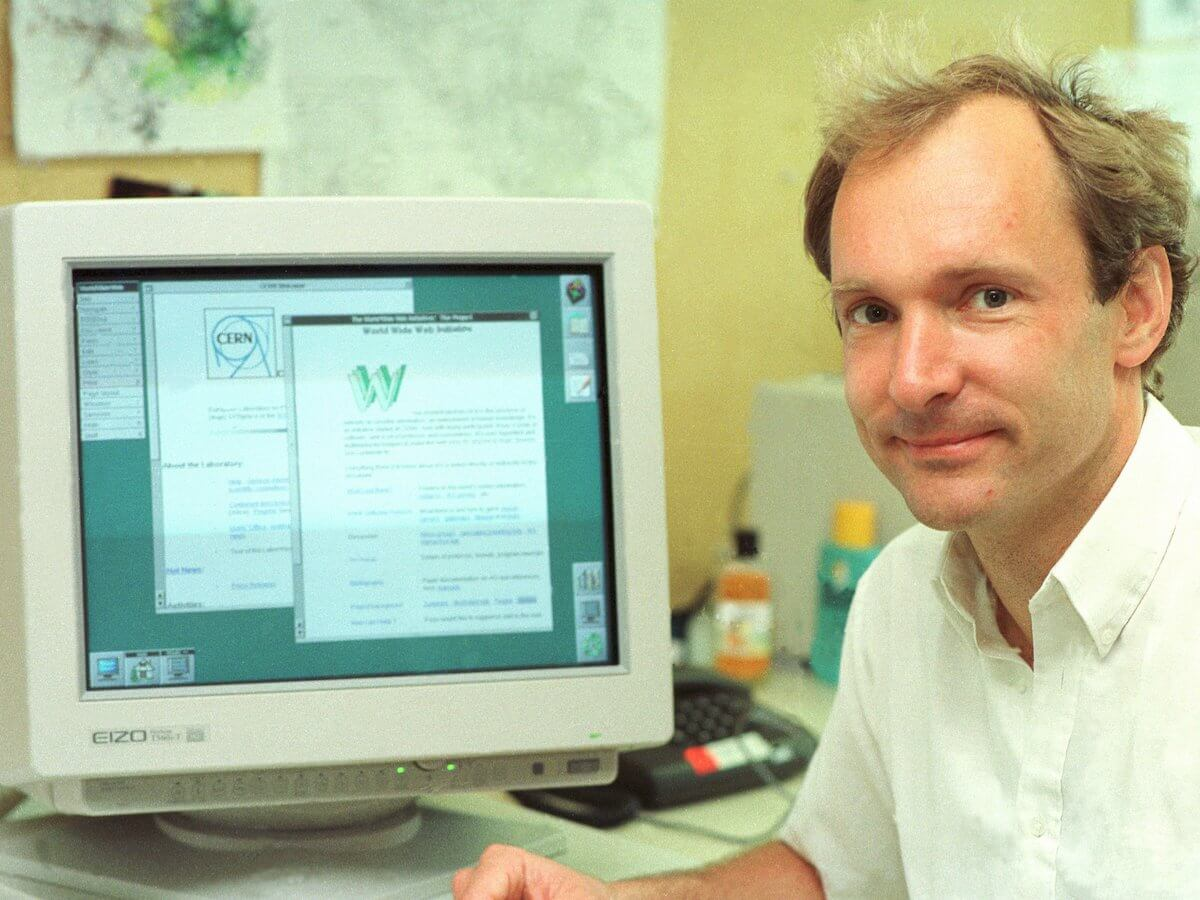
\includegraphics[width=0.87
	\textwidth,  keepaspectratio]{fig/Berners-Lee}
	\caption{Sir Tim Berners-lee, fondatore del {\tt World Wide Web}, davanti al primo prototipo di browser.}
	\label{fig:bernersLee}
\end{figure}

\medskip 

Sir Tim Berners-Lee, fondatore del {\tt World Wide Web} e del progetto {\tt Solid}, insignito del premio Turing nel 2016, con il passare degli anni fu mosso da una crescente preoccupazione relativa al modo con cui la sua creazione, il {\tt WWW}, si era evoluta. Con il passare del tempo iniziò a dubitare del reale beneficio apportato da questa tecnologia alla società umana \cite{sciencefocus}.

\bigskip

Nella visione di Berners-Lee, il {\tt World Wide Web} sarebbe dovuto essere un luogo in cui tutti gli utenti, attraverso un meccanismo di autorizzazioni, avrebbero potuto collaborare per creare nuovi contenuti sulla rete. Infatti, il primo browser della storia, sviluppato nel {\tt CERN} di Ginevra, era stato progettato per essere anche un editor, con il fine di permettere uno scambio di dati in maniera decentralizzata tra utenti. Tuttavia la prima versione di browser che rese il web popolare tagliò questa funzionalità, poiché ritenuta troppo difficile da implementare.  

\bigskip
\bigskip

Berners-Lee, il 12 marzo 2017, in occasione del ventottesimo compleanno di internet, delineò i tre principali problemi principali relativi alla sua creazione \cite{worldwideweb}:

\bigskip
\bigskip

\textbf{"We’ve lost control of our personal data"}. Gli utenti di Internet accettano di utilizzare servizi gratuitamente in cambio della cessione dei loro dati personali; questo ha portato le grandi multinazionali, come i più importanti social network, a collezionare i dati dei loro utenti per fini personali. Società e governi hanno iniziato a osservare i movimenti online degli tali utenti, portando, ad esempio, all'arresto e all'uccisione di alcuni cittadini in Paesi vittime di regimi dittatoriali. \cite{bloggers}

\bigskip
\bigskip

\textbf{"It’s too easy for misinformation to spread on the web"}. Tramite i dati raccolti dagli utenti, attraverso l'utilizzo di appositi algoritmi, i social network possono mostrare contenuti in base ai loro interessi, inviando loro link ad altri siti web. Tali siti spesso risultano essere fonti di disinformazione o di fake news e mostrano all'utente contenuti in base alle sue credenze e ai suoi pregiudizi in modo da condizionarne le idee \cite{nyt}\label{key}.

\bigskip
\bigskip

\textbf{"Political advertising online needs transparency and understanding"}. Berners-Lee ha infine evidenziato i problemi connessi con l'industria delle publicità politiche. Tramite i dati degli utenti, i quali vengono continuamente raccolti dai social network, vengono create pubblicità individuali rivolte ai singoli, in base ai loro dati. É stato stimato da una fonte \cite{guardian} che, durante le elezioni presidenziali degli Stati Uniti d'America del 2016, siano state create ogni giorno circa 50.000 variazioni di pubblicità di natura politica con il fine di renderle più adatte ai singoli utenti. Berners-Lee ritenne che vi fossero molti indizi sulla non eticità di tali pubblicità.

\bigskip
\bigskip

Le preoccupazioni di Berners-Lee si sono ulteriormente acuite a seguito dello scandalo Facebook-Cambridge Analytica, avvenuto nel 2018. Tale scandalo mise in evidenza che il noto social network Facebook aveva raccolto dati di 87 milioni di utenti senza il loro consenso per scopi di propaganda politica \cite{facebook}. 

\bigskip

\section{Nascita del progetto Solid}

\medskip

Queste considerazioni hanno portato alla nascita del progetto {\tt Solid} da parte di {\tt Berners-Lee}. Egli mira a superare le problematiche elencate rendendo gli utenti i veri proprietari del web, ridecentralizzandolo, come quando lo aveva originariamente creato \cite{techchahiye}.

\medskip

Il progetto nasce già nel 2015 in collaborazione con il {\tt MIT}; allo sviluppo di questa tecnologia hanno collaborato anche l'Università di Oxford e l'Istituto di Ricerca Informatica del Qatar. Nel 2018 Berners-Lee si prende un anno sabbatico dal progetto per fondare la società {\tt Inrupt}, già menzionata nel capitolo 2, con il fine di mettere a disposizione degli sviluppatori strumenti per poter interagire con {\tt Solid}.

\medskip

Come in parte già descritto, {\tt Solid} mira a risolvere i problemi evidenziati da Berners-Lee, cambiando il modello attuale di consegna dei propri dati ai giganti informatici in cambio dell'accesso ad alcuni servizi, poiché tale modello penalizza gli utenti del web, privandoli della loro privacy. {\tt Solid} mira ad evolvere il web riequilibrandolo, dando ad ognuno il completo controllo dei propri dati, personali e non, in modo innovativo. Berners-Lee è fermamente convinto riguardo la necessarietà di {\tt Solid} per poter modificare il web, sostenendo che, tramite questa tecnologia le persone riusciranno a riprendersi il loro potere dalle grandi corporazioni. A tal proposito Berners-Lee ha dichiarato: "Non stiamo chiedendo a Facebook o a Google se introdurre o meno un completo cambiamento (sul web) che porterà a capovolgere completamente il loro modello di business, non stiamo chiedendo a loro permessi" \cite{fastcompany}.


\bigskip

\section{Nascita del sistema SADeB}

\medskip

Il sistema {\tt SADeB} (Solid Authenticity Decentralized Blog) nasce con l'intento di mettere in evidenza le potenzialità della tecnologia {\tt Solid}, mostrando le differenze tra l'applicazione {\tt Solid} {\tt my-solid-blog} e un normale social network.

\medskip

Come già descritto, le applicazioni {\tt Solid} sono totalmente svincolate dai dati che mostrano all'utente con cui interagiscono; ciò permette all'utente stesso di controllare i propri dati in maniera diretta, di comprendere chi li sta utilizzando e di permettere che questi vengano riutilizzati da più applicazioni differenti in base alle sue necessità. 

\medskip

La decentralizzazione effettuata da {\tt Solid} permette, inoltre, di tutelare l'utente che utilizza tali applicazioni, arginando in parte il problema relativo alla diffusione di disinformazione, evidenziato anche da Berners-Lee stesso \cite{worldwideweb}. Infatti, tramite {\tt Solid}, è possibile implementare in maniera semplice ed efficiente dei controlli sull'autenticità dei dati mostrati all'utente. L'applicazione {\tt blog-validator}, facente parte del sistema {\tt SADeB}, si occupa, infatti, di controllare che l'applicazione {\tt my-solid-blog} non abbia volontariamente modificato i dati contenuti all'interno del {\tt Pod} dell'utente, con il fine di diffondere informazioni false. {\tt blog-validator} si occupa quindi di comparare i dati visualizzati da {\tt my-solid-blog} con quelli realmente presenti all'interno del {\tt Pod} dell'utente, indicando, eventualmente a quest'ultimo, se tali dati siano stati modificati. {\tt blog-validator} è un'applicazione esterna e svincolata da {\tt my-solid-blog}, creata per poter essere utilizzata, apportando alcune modifiche al codice in base alle necessità, non solo da {\tt my-solid-blog}, ma anche da altre possibili applicazioni decentralizzate, per dare garanzie ai loro utenti riguardo la validità delle informazione loro mostrate.

\clearpage